\documentclass[sigconf]{acmart}

% rights management commands, sent to the author by ACM after rights form completion.

\copyrightyear{2026}
\acmYear{2026}
\setcopyright{cc}
\setcctype{by}
\acmConference[I3D Companion '26]{Companion Proceedings of the Symposium on Interactive 3D Graphics and Games}{May 13--15, 2026}{San Francisco, CA, USA}
\acmBooktitle{Companion Proceedings of the Symposium on Interactive 3D Graphics and Games (I3D Companion '26), May 13--15, 2026, San Francisco, CA, USA}
\acmDOI{10.1145/3807895.3807935}
\acmISBN{979-8-4007-2667-5/2026/05}

% packages to add, making sure they are in https://authors.acm.org/proceedings/production-information/accepted-latex-packages.

\usepackage{graphicx}
\usepackage{subfig}

% Submission ID.
% Use this when submitting an article to a sponsored event. You'll receive a unique submission ID from the organizers of the event, 
% and this ID should be used as the parameter to this command.
\acmSubmissionID{19}

% reference and citation style.
\citestyle{acmauthoryear}

\begin{document}

\author{James Youngblood}
\affiliation{
  \institution{University of Utah}
  \city{Salt Lake City}
  \state{UT}
  \country{USA}}
\email{james@youngbloods.org}

\author{Rogelio E. Cardona-Rivera}
\affiliation{
	\department{Division of Games}
	\institution{University of Utah}
  \city{Salt Lake City}
	\state{UT}
  \country{USA}}
\email{r.cardona.rivera@utah.edu}

\title{Reliability of Gaze Prediction for Stylized and Transformed Images}

% CCS Concepts. Required for any ACM work over two pages in length.
% Visit http://dl.acm.org/ccs and generate this content for your work.

\begin{CCSXML}
	<ccs2012>
	<concept>
	<concept_id>10010147.10010178.10010224.10010245.10010246</concept_id>
	<concept_desc>Computing methodologies~Interest point and salient region detections</concept_desc>
	<concept_significance>500</concept_significance>
	</concept>
	<concept>
	<concept_id>10010147.10010257.10010339</concept_id>
	<concept_desc>Computing methodologies~Cross-validation</concept_desc>
	<concept_significance>500</concept_significance>
	</concept>
	<concept>
	<concept_id>10010147.10010257.10010293.10010294</concept_id>
	<concept_desc>Computing methodologies~Neural networks</concept_desc>
	<concept_significance>100</concept_significance>
	</concept>
	<concept>
	<concept_id>10010147.10010371.10010387.10010393</concept_id>
	<concept_desc>Computing methodologies~Perception</concept_desc>
	<concept_significance>300</concept_significance>
	</concept>
	<concept>
	<concept_id>10010147.10010371.10010382.10010383</concept_id>
	<concept_desc>Computing methodologies~Image processing</concept_desc>
	<concept_significance>500</concept_significance>
	</concept>
	<concept>
	<concept_id>10010147.10010371.10010372.10010375</concept_id>
	<concept_desc>Computing methodologies~Non-photorealistic rendering</concept_desc>
	<concept_significance>300</concept_significance>
	</concept>
	</ccs2012>
\end{CCSXML}

\ccsdesc[500]{Computing methodologies~Interest point and salient region detections}
\ccsdesc[500]{Computing methodologies~Cross-validation}
\ccsdesc[500]{Computing methodologies~Image processing}
\ccsdesc[300]{Computing methodologies~Perception}
\ccsdesc[300]{Computing methodologies~Non-photorealistic rendering}
\ccsdesc[100]{Computing methodologies~Neural networks}

\keywords{saliency map, visual attention, generalizability, visual fixation prediction}

\begin{abstract}
Recent advancements have shown increasingly accurate and fast visual gaze prediction models, which might now be feasible for real-time scenarios. These gaze prediction models would allow a program to infer where a user might focus on in an rendered scene, and might allow unique program behavior, rendering optimizations based on perception, or modelling of the user's visual attention, without requiring direct eye-tracking hardware. Current state-of-the-art models use deep learning techniques, and most published image data sets for training are biased towards photography, at the expense of computer-rendered scenes, especially those with stylized subjects. We raise concerns over the generalizability of state-of-the-art models. We study a number of digital image transformations on existing datasets, using them as a reference point for what various rendering techniques or stylization effects might have on gaze prediction models. Our findings show that state-of-the-art models perform significantly worse on common image transformations. Our experiments reveal no significant, computable indicators of loss in accuracy, meaning more human gaze distribution data must be gathered in order to train and validate the generalizability of gaze prediction models.
\end{abstract}

\maketitle

\section{Introduction}
Recent years have seen many advancements in the field of visual fixation prediction, which is the
task of predicting the points at which a human will first focus on within the area of an image
(sometimes called the "saliency" of an image). Droste et al. provide a new gaze prediction
model, called UNISAL \cite{unisal}, which is among the top performing models on the MIT-Tuebingen
Saliency Benchmark \cite{mit-tuebingen}, and which generates predictions on frames in the DHF1K
\cite{dhf1k} dataset in nine milliseconds, moving gaze prediction tasks into the realm of real-time
computing.

The most prominent published data sets for image saliency, including the MIT 300 \cite{mit300} and
CAT 2000 \cite{cat2000}, provide only a handful of 3D computer-rendered scenes. Even the amount of
stylized art, such as painting and collage, is noticeably lesser than that of photos of
physical subjects in these datasets. The report from Kümmerer et al. \cite{annurev-vision} shows that
leading gaze prediction models use deep-learning techniques, and the black-box nature of these
techniques raises concerns that the models will not generalize well to all classes of images,
especially those which are under-represented in the training data set.

\begin{figure}%
    \centering
    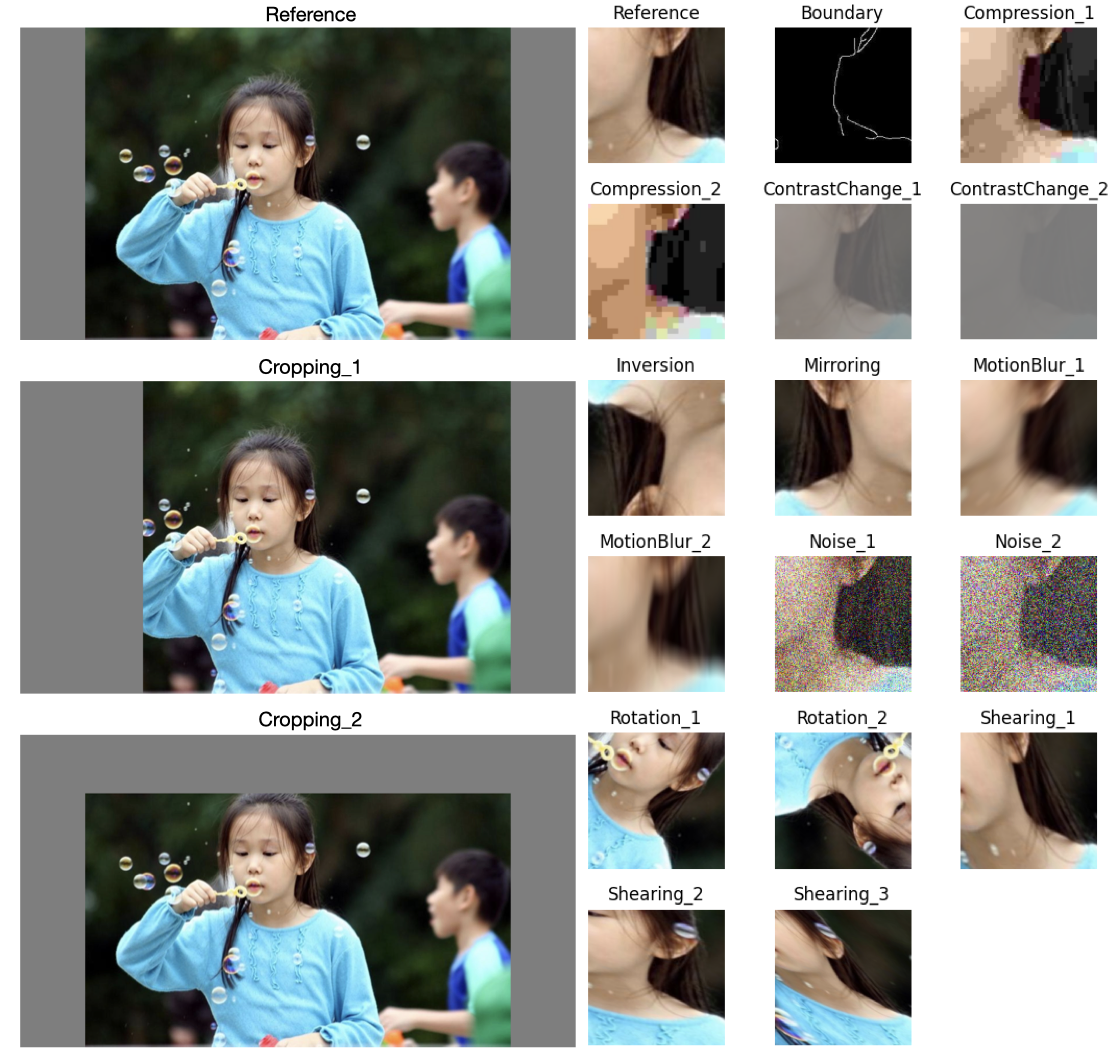
\includegraphics[width=8cm]{all_examples.png}
		\caption{Shown are examples for each transformation we study, applied to the image labelled as the reference. These examples provide an intuition for the visual qualities and intensity of each transformation. Each transformation is labeled.}
		\Description{Several images are displayed which demonstrate the visual characteristics of transformations we study. The images include the reference image, as well as the images for boundary, compression, contrast change, cropping, mirroring, motion blur, gaussian noise, rotation, and shearing transformations.}
    \label{fig:examples}%
\end{figure}

\section{Method}
Although we wish to study model accuracy on computer-rendered images against benchmark results,
we realize that it is difficult to isolate against the effects of uncontrolled variables when
comparing two differing data sets. Instead, we hypothesize that digital transformations of a set
of images, when compared to the untransformed images, will degrade the model's predictive
accuracy. We assume that by showing common digital transformations degrade accuracy, we show
that the models cannot be expected to generalize well to many other domains of images,
including stylized and computer-rendered images, especially those which have visual
similarities to the transformations we test.

We utilize the dataset produced by Che et al. \cite{gaze-transformations}, which randomly selects 100
images from the CAT 2000 \cite{cat2000} dataset, produces corresponding transformed images for 18
transformation types (demonstrated in Figure \ref{fig:examples}), and measures gaze distributions of human subjects for all 1900 images. For
each image, we measure the model's score on the NSS \cite{nss} and IG \cite{information-gain} metrics, and express
those scores as percentages of the "gold standard" minus the "center bias" scores. The gold
standard and the center bias are are described by Kümmerer et al. \cite{information-gain} to be the
"best guess" for an image with all image-specific human gaze data considered, and with only
dataset-specific human gaze data considered, respectively. Together, they provide a good upper
bound and lower reference point with which to consider a model's prediction accuracy.
Expressing scores within this range allows us to find model degradation beyond that which might
be expected due to a destructive or non-reversible transformation, as the degradation in
performance produced by any destructive transformation should be captured by the gold standard
and center bias for that transformation.

\section{Results}
We find that for both DeepGaze IIE \cite{deepgazeiie} and UNISAL models, which hold top spots
on the MIT-Tuebingen Saliency benchmark, the overwhelming majority of transformations suffer
significant loss (listed in Table \ref{tab:results}) for both IG and NSS metrics, relative to
untransformed images. The UNISAL model in particular can suffer loss of over 100 percentage
points in the most extreme case. Untransformed images perform roughly in line with benchmark
expectations, while almost all transformed images degrade to some degree beyond that which can be
expected by loss of information during the transformation. These findings support our hypothesis,
and seem to indicate that current models have poor generalizability to stylized images which bear
resemblance to the common transformations we tested (including cropping, gaussian noise, contrast
adjustment, rotation, shearing, motion blur, and edge enhancement).

\begin{table}
	\caption{The change in prediction accuracy is shown for the NSS and IG metrics on both DeepGaze IIE
	and UNISAL models. Each listed percentage change represents the difference between transformation
	and reference median metric scores represented as a percentage of the center-bias/gold standard
	range.}
	\label{tab:results}
	\begin{small}
		\begin{tabular}{lcccc}%
			\toprule
			& \multicolumn{2}{c}{DeepGaze IIE} & \multicolumn{2}{c}{UNISAL} \\
			Transformation & NSS & IG & NSS & IG \\
			\midrule
			Reference & 0.00\% & 0.00\% & 0.00\% & 0.00\% \\
			Boundary & -6.27\% & -6.56\% & -25.67\% & -13.25\% \\
			Compression\_1 & -19.52\% & -13.31\% & -26.62\% & -5.98\% \\
			Compression\_2 & -13.99\% & -23.46\% & -23.33\% & -7.86\% \\
			ContrastChange\_1 & 1.33\% & 5.17\% & -23.00\% & -18.05\% \\
			ContrastChange\_2 & -35.82\% & -25.86\% & -43.70\% & -48.18\% \\
			Cropping\_1 & -20.65\% & -13.41\% & -16.26\% & -13.97\% \\
			Cropping\_2 & -22.15\% & -11.90\% & -29.11\% & -13.46\% \\
			Inversion & -34.51\% & -20.98\% & -45.21\% & -28.10\% \\
			Mirroring & -7.16\% & 4.82\% & -10.23\% & 0.16\% \\
			MotionBlur\_1 & -50.47\% & -45.27\% & -41.18\% & -32.08\% \\
			MotionBlur\_2 & -75.38\% & -49.91\% & -75.50\% & -41.12\% \\
			Noise\_1 & -7.39\% & -15.94\% & -8.81\% & -11.73\% \\
			Noise\_2 & -18.63\% & -19.64\% & -26.61\% & -24.72\% \\
			Rotation\_1 & -18.21\% & -39.90\% & -65.28\% & -70.90\% \\
			Rotation\_2 & -39.61\% & -25.03\% & -128.33\% & -93.75\% \\
			Shearing\_1 & -20.93\% & -16.63\% & -28.30\% & -26.53\% \\
			Shearing\_2 & 3.77\% & -2.95\% & -43.73\% & -37.03\% \\
			Shearing\_3 & -13.88\% & -30.50\% & -63.48\% & -66.06\% \\
			\bottomrule
		\end{tabular}
	\end{small}
\end{table}

\section{Conclusion}
Our work indicates that state-of-the-art gaze prediction models cannot be relied on to produce
predictions that are as accurate as benchmarks profess for images that are not well represented
by prominent saliency data sets. This includes stylized and computer-rendered images. Unlocking
gaze prediction for real-time rendering applications will likely require much greater amounts of
training data and validation studies for these models.

Code for model inference, metric computation, and visualization of data; as well as plaintext data
for our results; have been published as supplementary material, and can also be found at our
repository \cite{our-code}.

\bibliographystyle{ACM-Reference-Format}
\bibliography{main}

\end{document}
